% This is the now Chapter 6
This section presents the comprehensive evaluation of the proposed multimodal approach for pedagogical assessment. The analysis compares the performance of individual modalities (visual, audio, and linguistic) against the combined multimodal approach using two machine learning algorithms: Logistic Regression and Support Vector Machine (SVM).

The experimental results demonstrate a clear superiority of the multimodal approach over individual modality-based assessments. Table~\ref{tab:performance_summary} presents the comprehensive performance metrics across all tested configurations.

\begin{figure}[H]
    \centering
    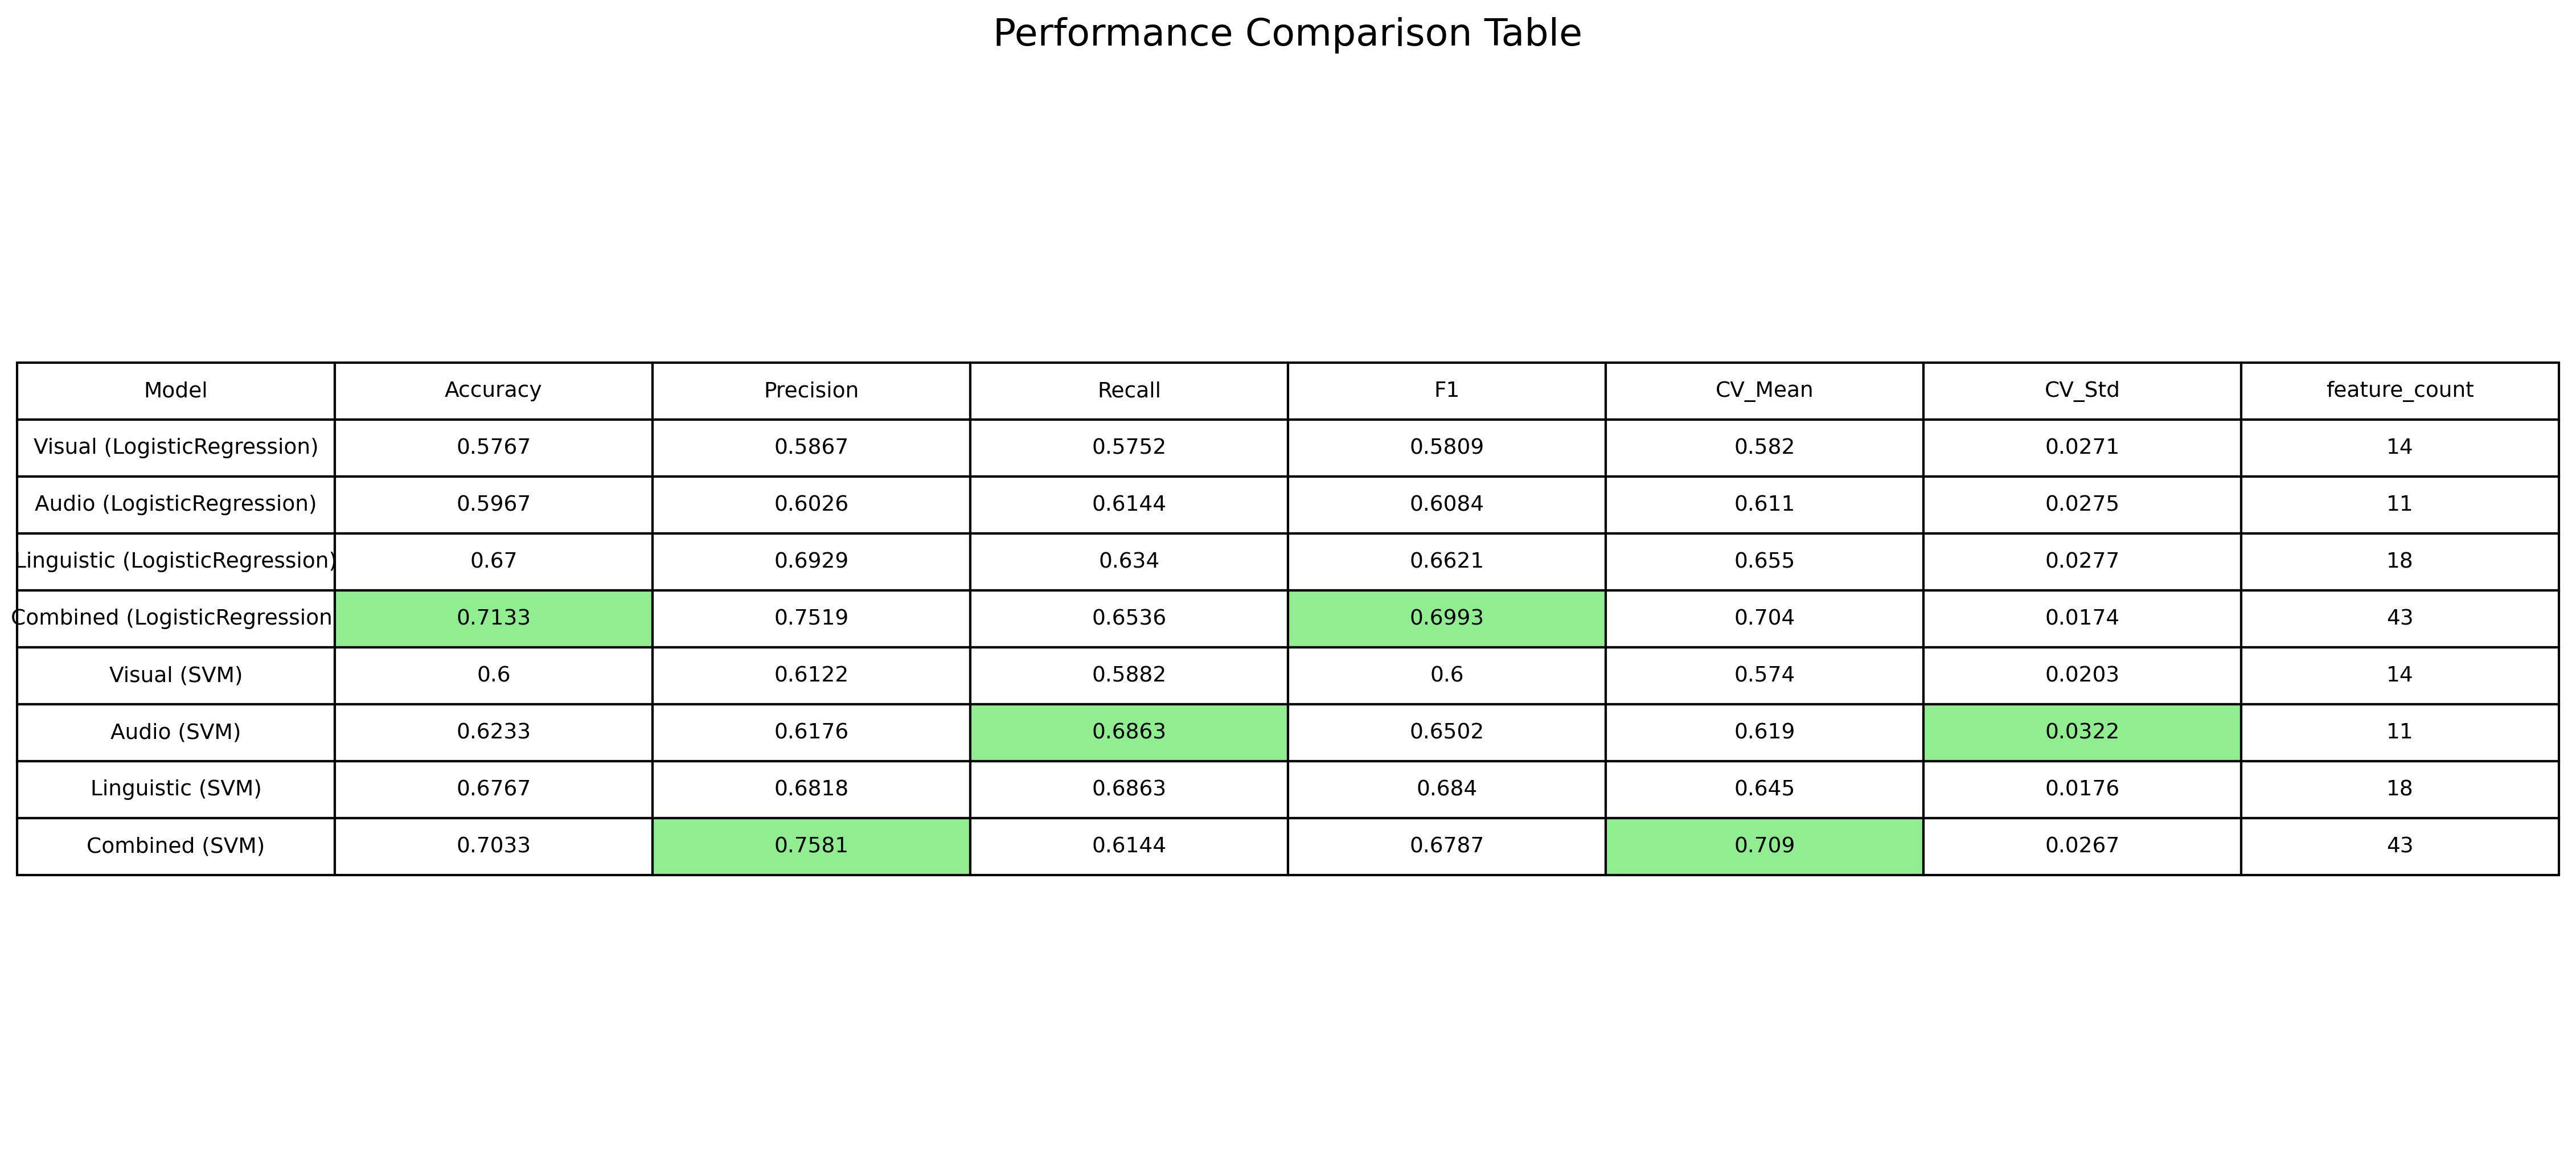
\includegraphics[width=0.9\textwidth]{sections/performance_table.jpg}
    \caption{Comprehensive Performance Comparison Table showing accuracy, precision, recall, F1-score, cross-validation means and standard deviations across all modality combinations and algorithms.}
    \label{fig:performance_table}
\end{figure}

The combined multimodal approach achieved the highest accuracy of 71.33\% using Logistic Regression, representing a substantial improvement over individual modalities. This finding strongly supports the central thesis that integrating multiple data sources provides a more comprehensive and accurate assessment of pedagogical outcomes.

\subsection{Individual Modality Analysis}

\subsubsection{Visual Features Performance}

Visual features, encompassing teacher movement patterns, gesture frequency, classroom coverage, and facial expressions, demonstrated moderate predictive capability. The Logistic Regression model achieved 57.67\% accuracy, while SVM reached 60.0\% accuracy for visual-only features.

Key visual indicators that contributed to the model's performance included:
\begin{itemize}
    \item Classroom coverage patterns reflecting teacher mobility and student engagement zones
    \item Frontal stance duration indicating direct student interaction
    \item Gesture frequency representing pedagogical expressiveness
    \item Spatial consistency measuring structured movement patterns
\end{itemize}

\subsubsection{Audio Features Performance}

Audio modality analysis focused on prosodic features, speech patterns, and vocal characteristics. This modality showed comparable performance to visual features, with Logistic Regression achieving 59.67\% accuracy and SVM reaching 62.33\% accuracy.

Critical audio features included:
\begin{itemize}
    \item Pitch variability indicating pedagogical emphasis and engagement
    \item Speech rate patterns reflecting content delivery pace
    \item Pause ratio analysis showing thoughtful discourse structure
    \item Intensity variations demonstrating vocal emphasis techniques
\end{itemize}

\subsubsection{Linguistic Features Performance}

Linguistic analysis proved to be the strongest individual modality, achieving 67.0\% accuracy with Logistic Regression and 67.67\% accuracy with SVM. This superior performance highlights the importance of discourse quality in pedagogical assessment.

Significant linguistic indicators comprised:
\begin{itemize}
    \item Lexical diversity reflecting vocabulary richness and adaptability
    \item Question ratio indicating interactive teaching approaches
    \item Use of examples and summaries showing structured content delivery
    \item Bloom's taxonomy complexity measuring cognitive engagement levels
\end{itemize}

\subsection{Multimodal Integration Results}

\begin{figure}[H]
    \centering
    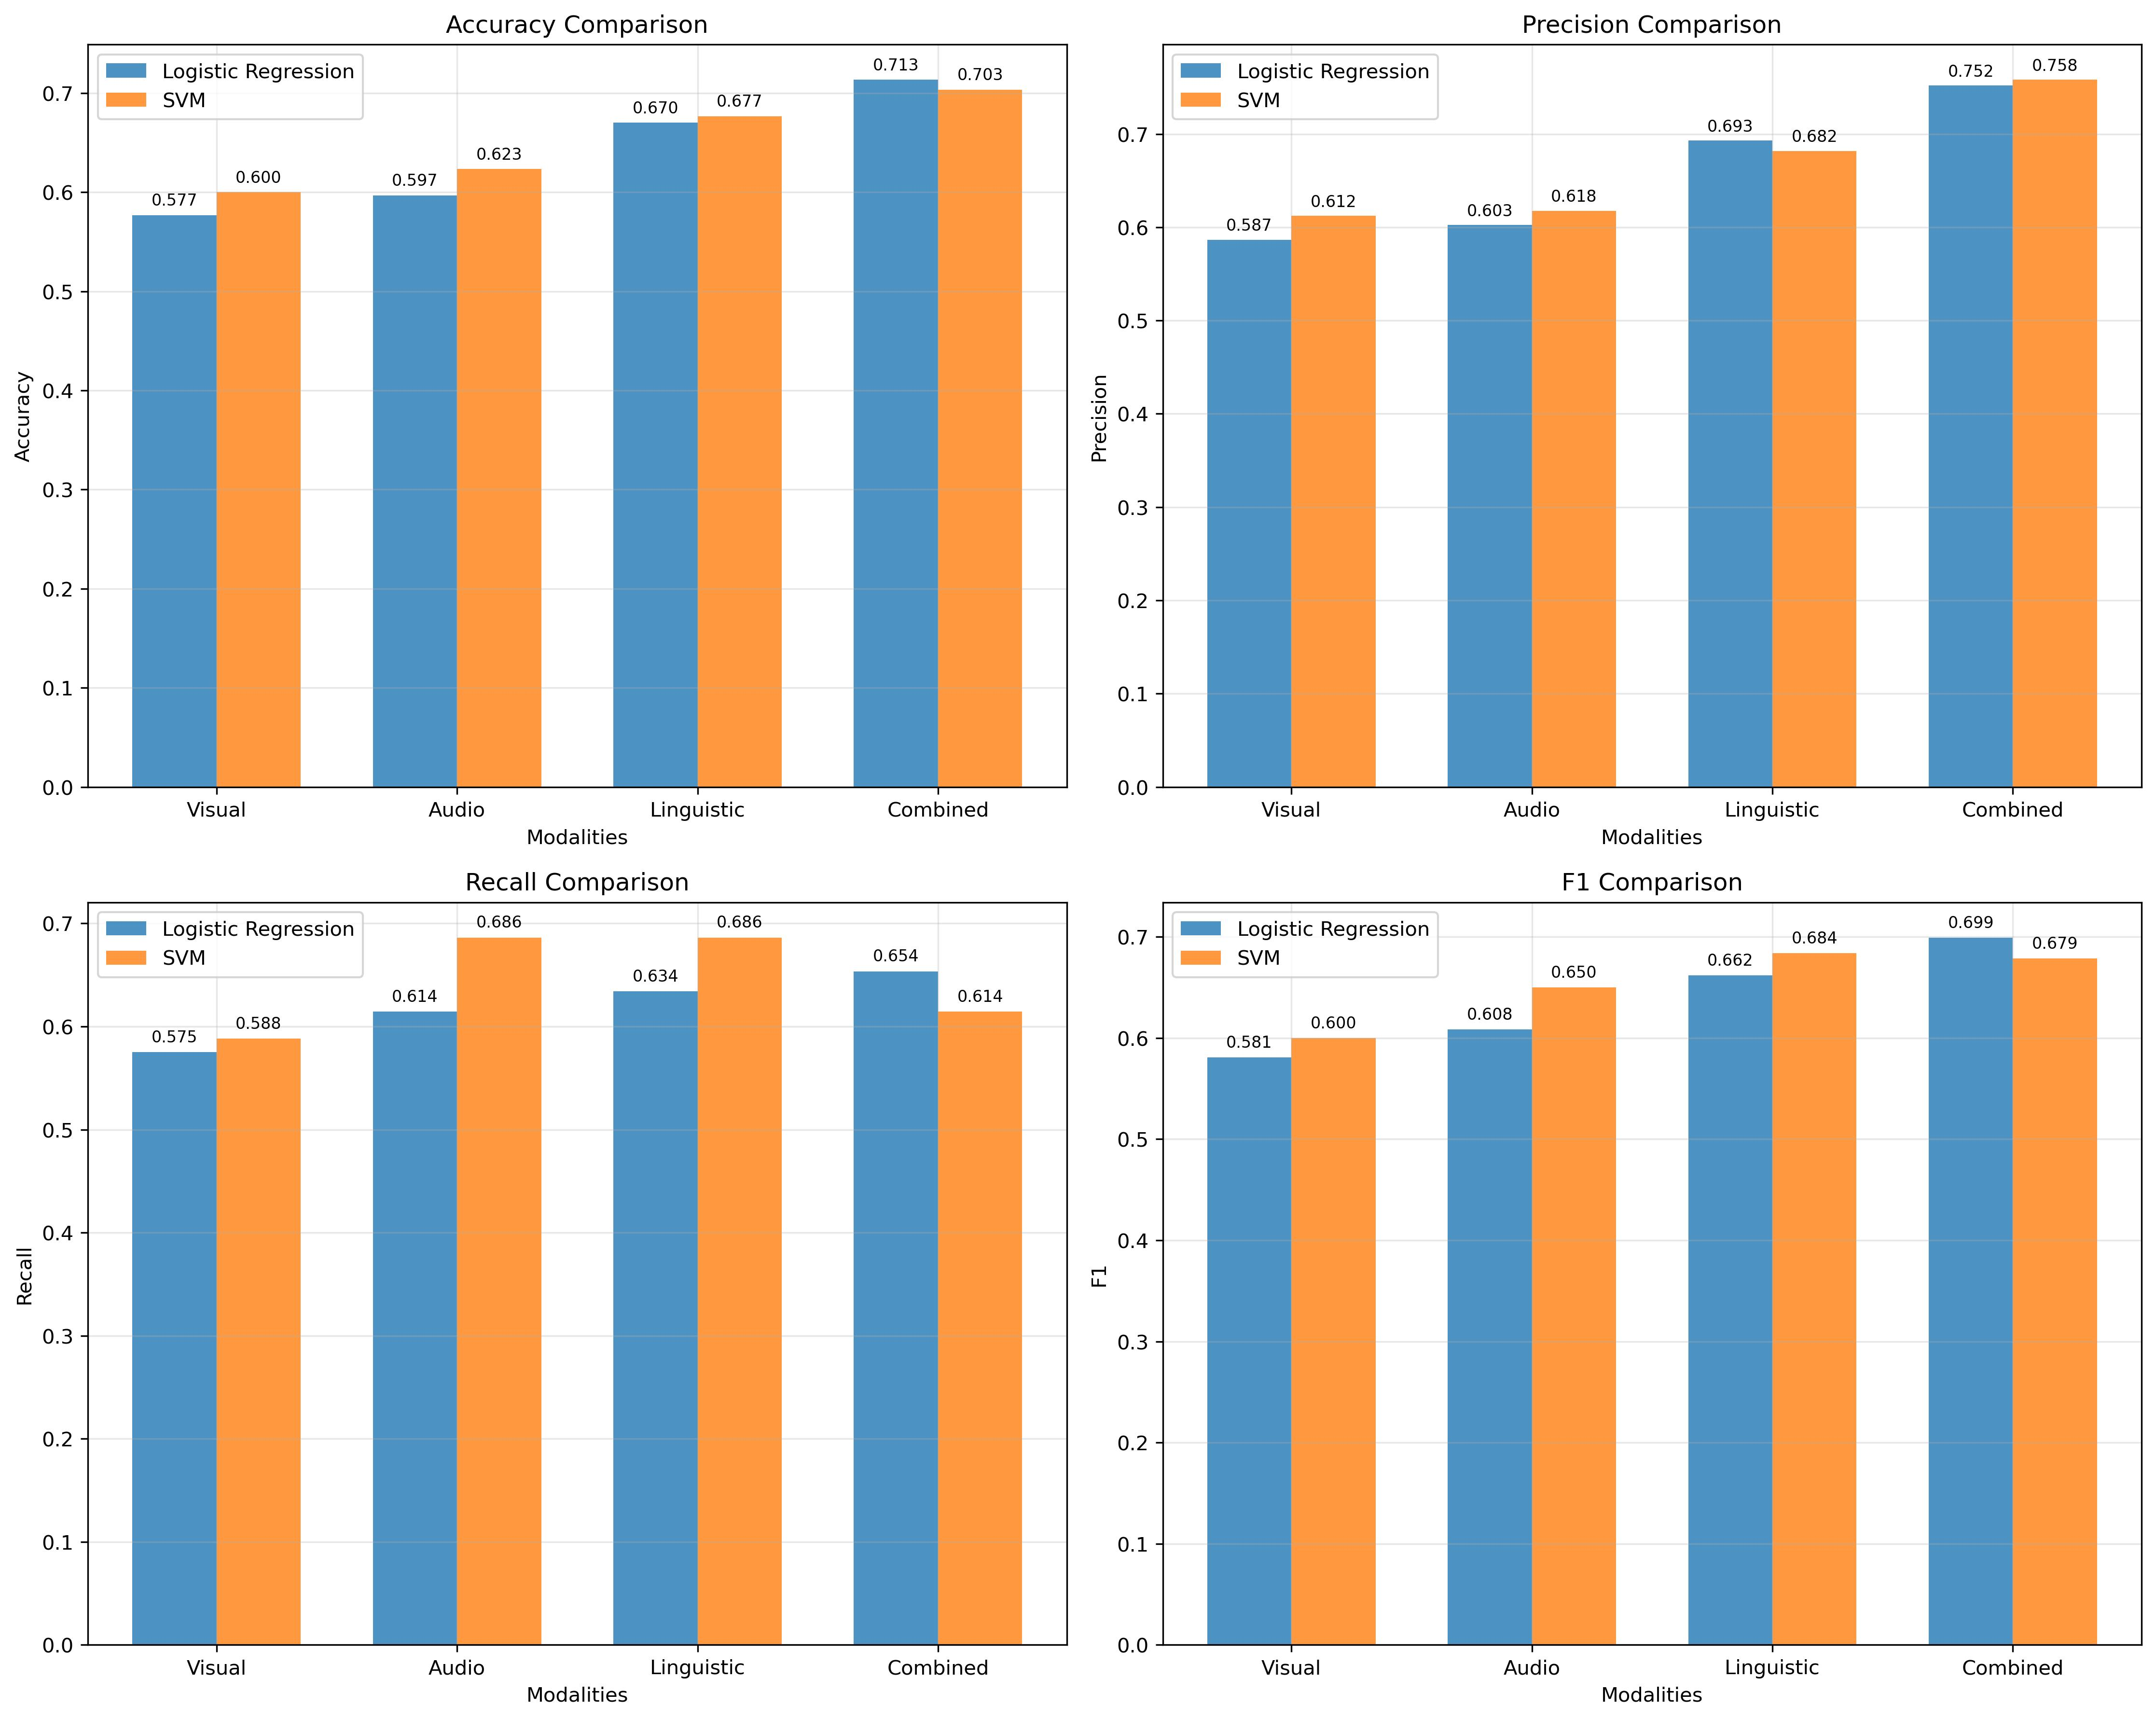
\includegraphics[width=\textwidth]{sections/performance_comparison.jpg}
    \caption{Performance comparison across all modalities and algorithms. The combined multimodal approach consistently outperforms individual modalities across all evaluation metrics (accuracy, precision, recall, and F1-score).}
    \label{fig:performance_comparison}
\end{figure}

The integration of all three modalities resulted in significant performance improvements. The combined approach achieved 71.33\% accuracy with Logistic Regression and 70.33\% accuracy with SVM, representing improvements of 4.33\% and 2.66\% respectively over the best individual modality (linguistic).

These improvements can be attributed to the complementary nature of different modalities:
\begin{itemize}
    \item \textbf{Visual-Audio Synergy:} Non-verbal cues complementing vocal emphasis patterns
    \item \textbf{Audio-Linguistic Correlation:} Prosodic features reinforcing discourse quality measures
    \item \textbf{Visual-Linguistic Alignment:} Physical positioning supporting pedagogical discourse strategies
\end{itemize}

\subsection{Cross-Validation Analysis}

\begin{figure}[H]
    \centering
    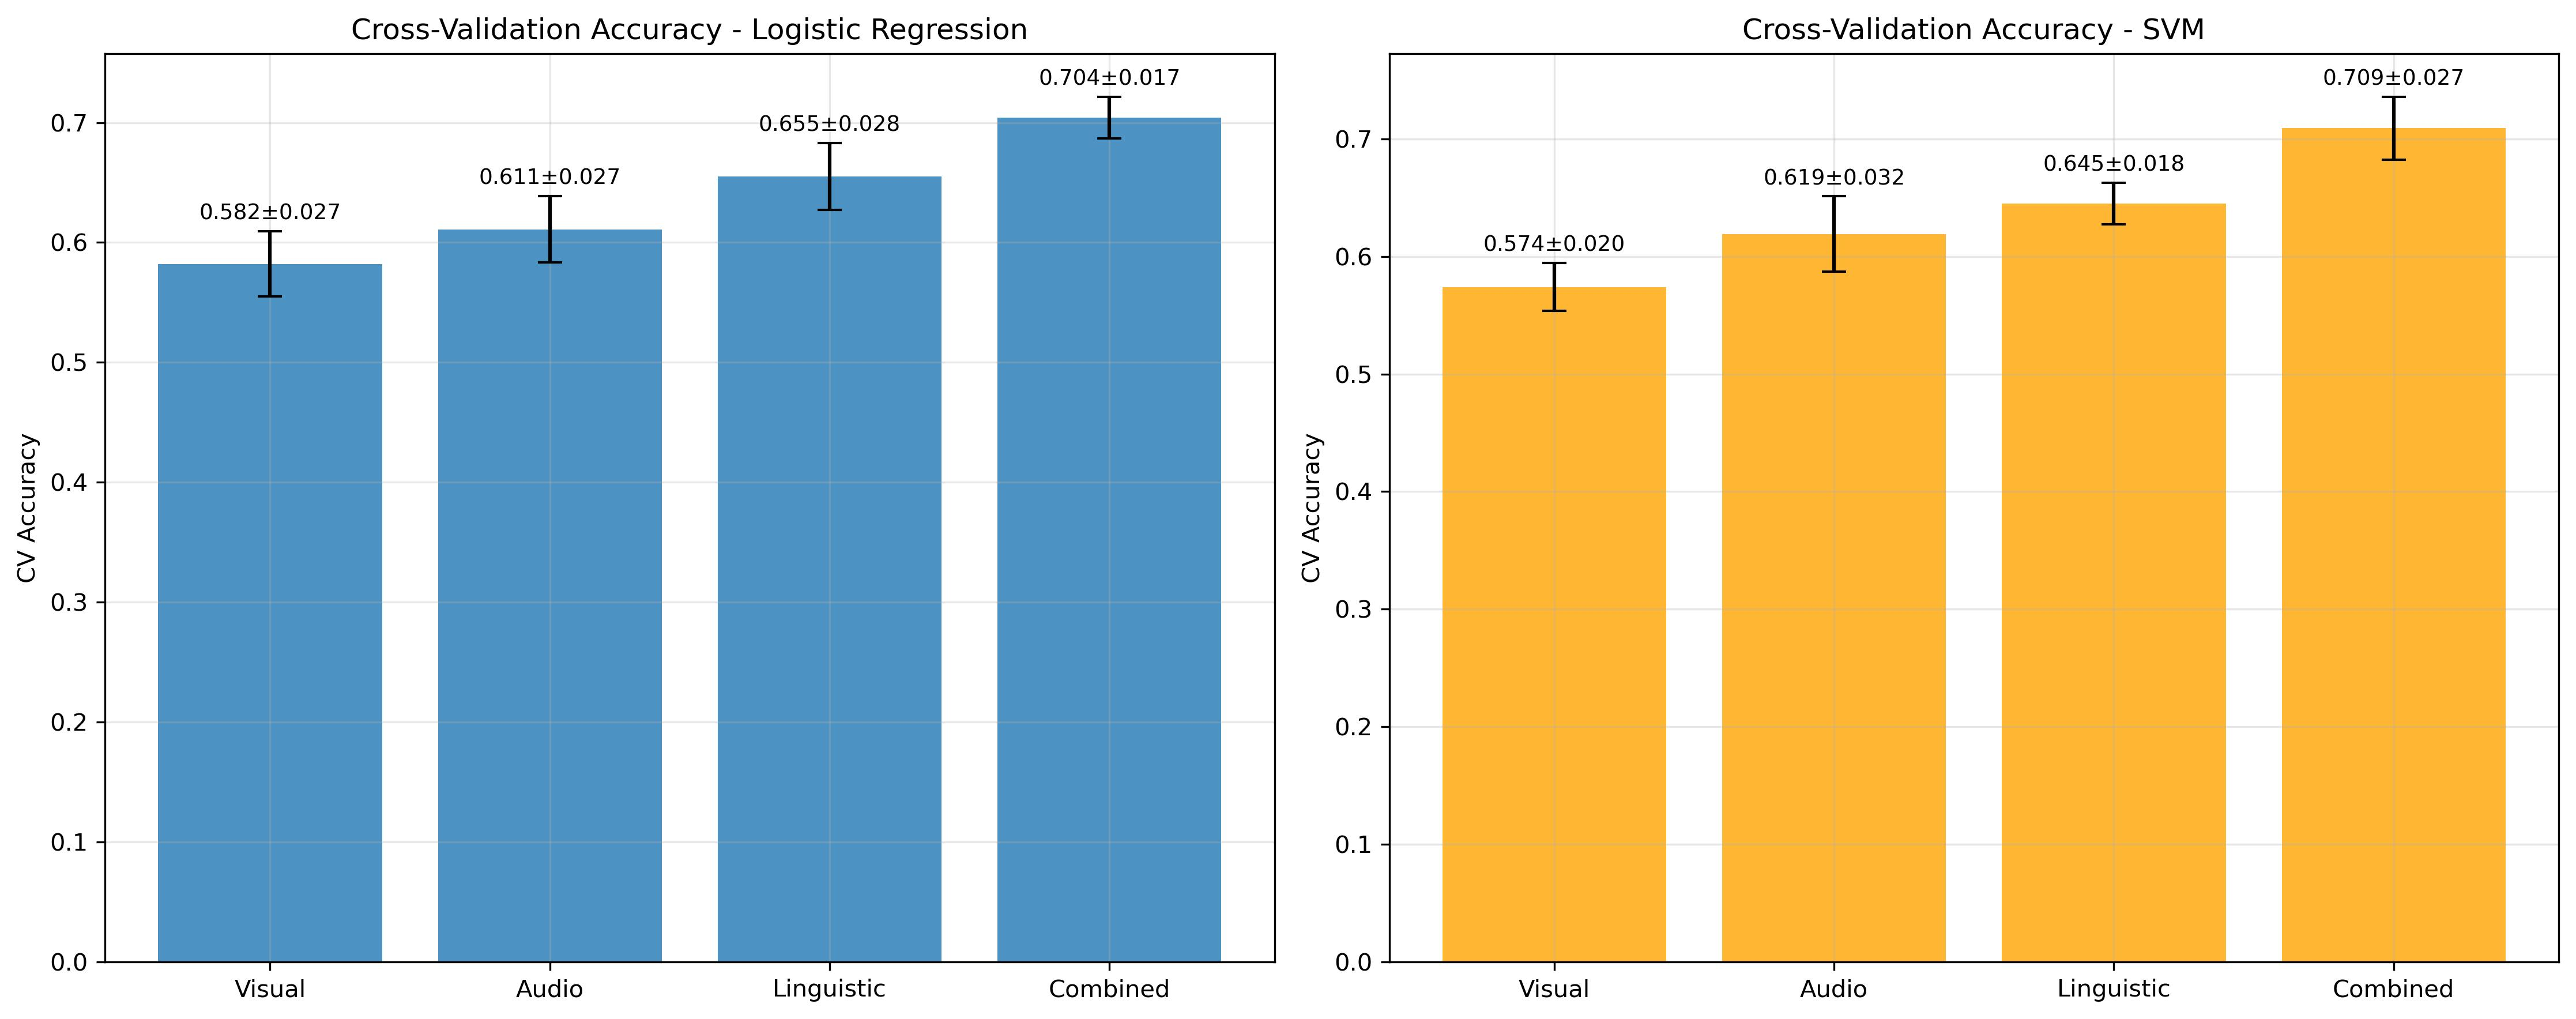
\includegraphics[width=\textwidth]{sections/cross_validation_comparison.jpg}
    \caption{Cross-validation accuracy results with error bars showing standard deviation. The multimodal approach demonstrates superior performance stability across both algorithms with reduced variance.}
    \label{fig:cross_validation}
\end{figure}

Cross-validation results provide robust evidence of the multimodal approach's superiority and stability. The combined approach achieved a mean cross-validation accuracy of 70.4\% (±1.74\%) for Logistic Regression and 70.9\% (±2.67\%) for SVM, with notably lower variance compared to individual modalities.

The reduced standard deviation in the multimodal approach indicates:
\begin{itemize}
    \item Enhanced model stability across different data splits
    \item Reduced overfitting through feature diversification
    \item More consistent performance across varying teaching contexts
\end{itemize}

\subsection{Feature Scaling and Model Performance}

\begin{figure}[H]
    \centering
    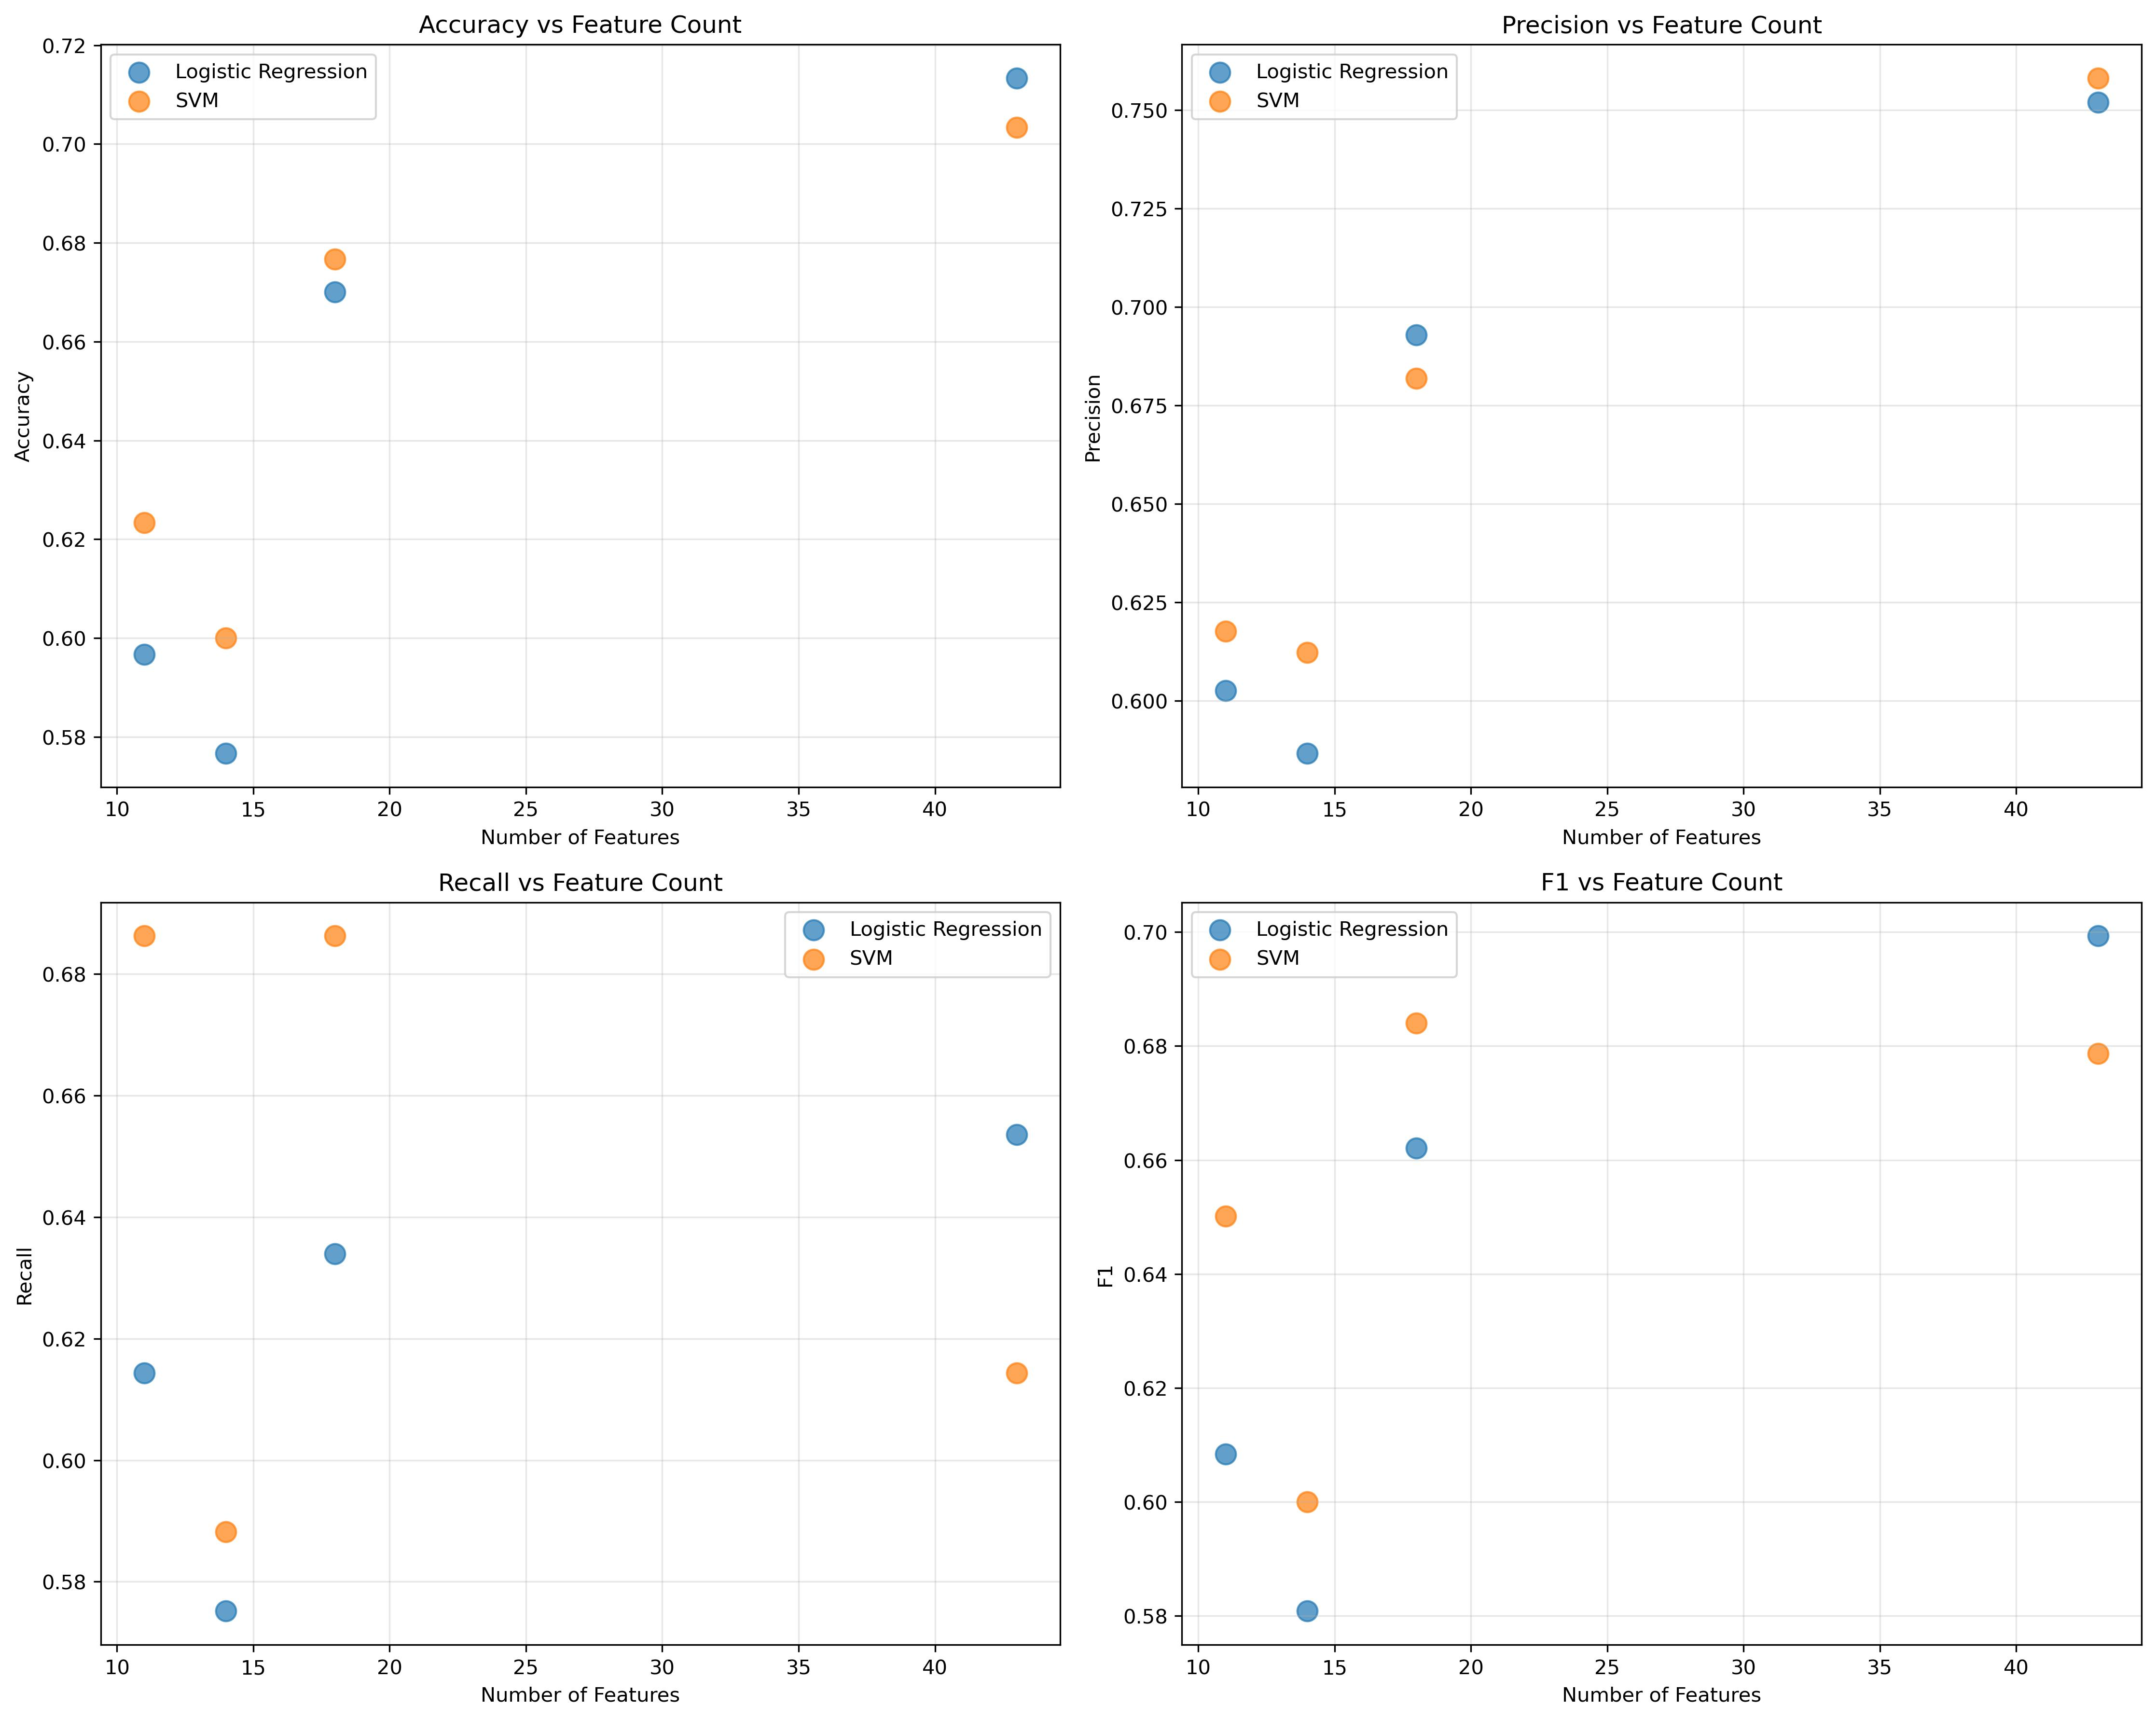
\includegraphics[width=\textwidth]{sections/feature_count_vs_performance.jpg}
    \caption{Relationship between feature count and model performance. The multimodal approach (43 features) demonstrates optimal performance gains, suggesting effective feature complementarity rather than mere feature accumulation.}
    \label{fig:feature_scaling}
\end{figure}

The analysis reveals that performance improvements are not merely due to increased feature dimensionality. While the combined approach utilizes 43 features compared to 11-18 features in individual modalities, the performance gains exceed what would be expected from simple feature addition, indicating genuine synergistic effects.

\subsection{Model Discrimination Capability}

\begin{figure}[H]
    \centering
    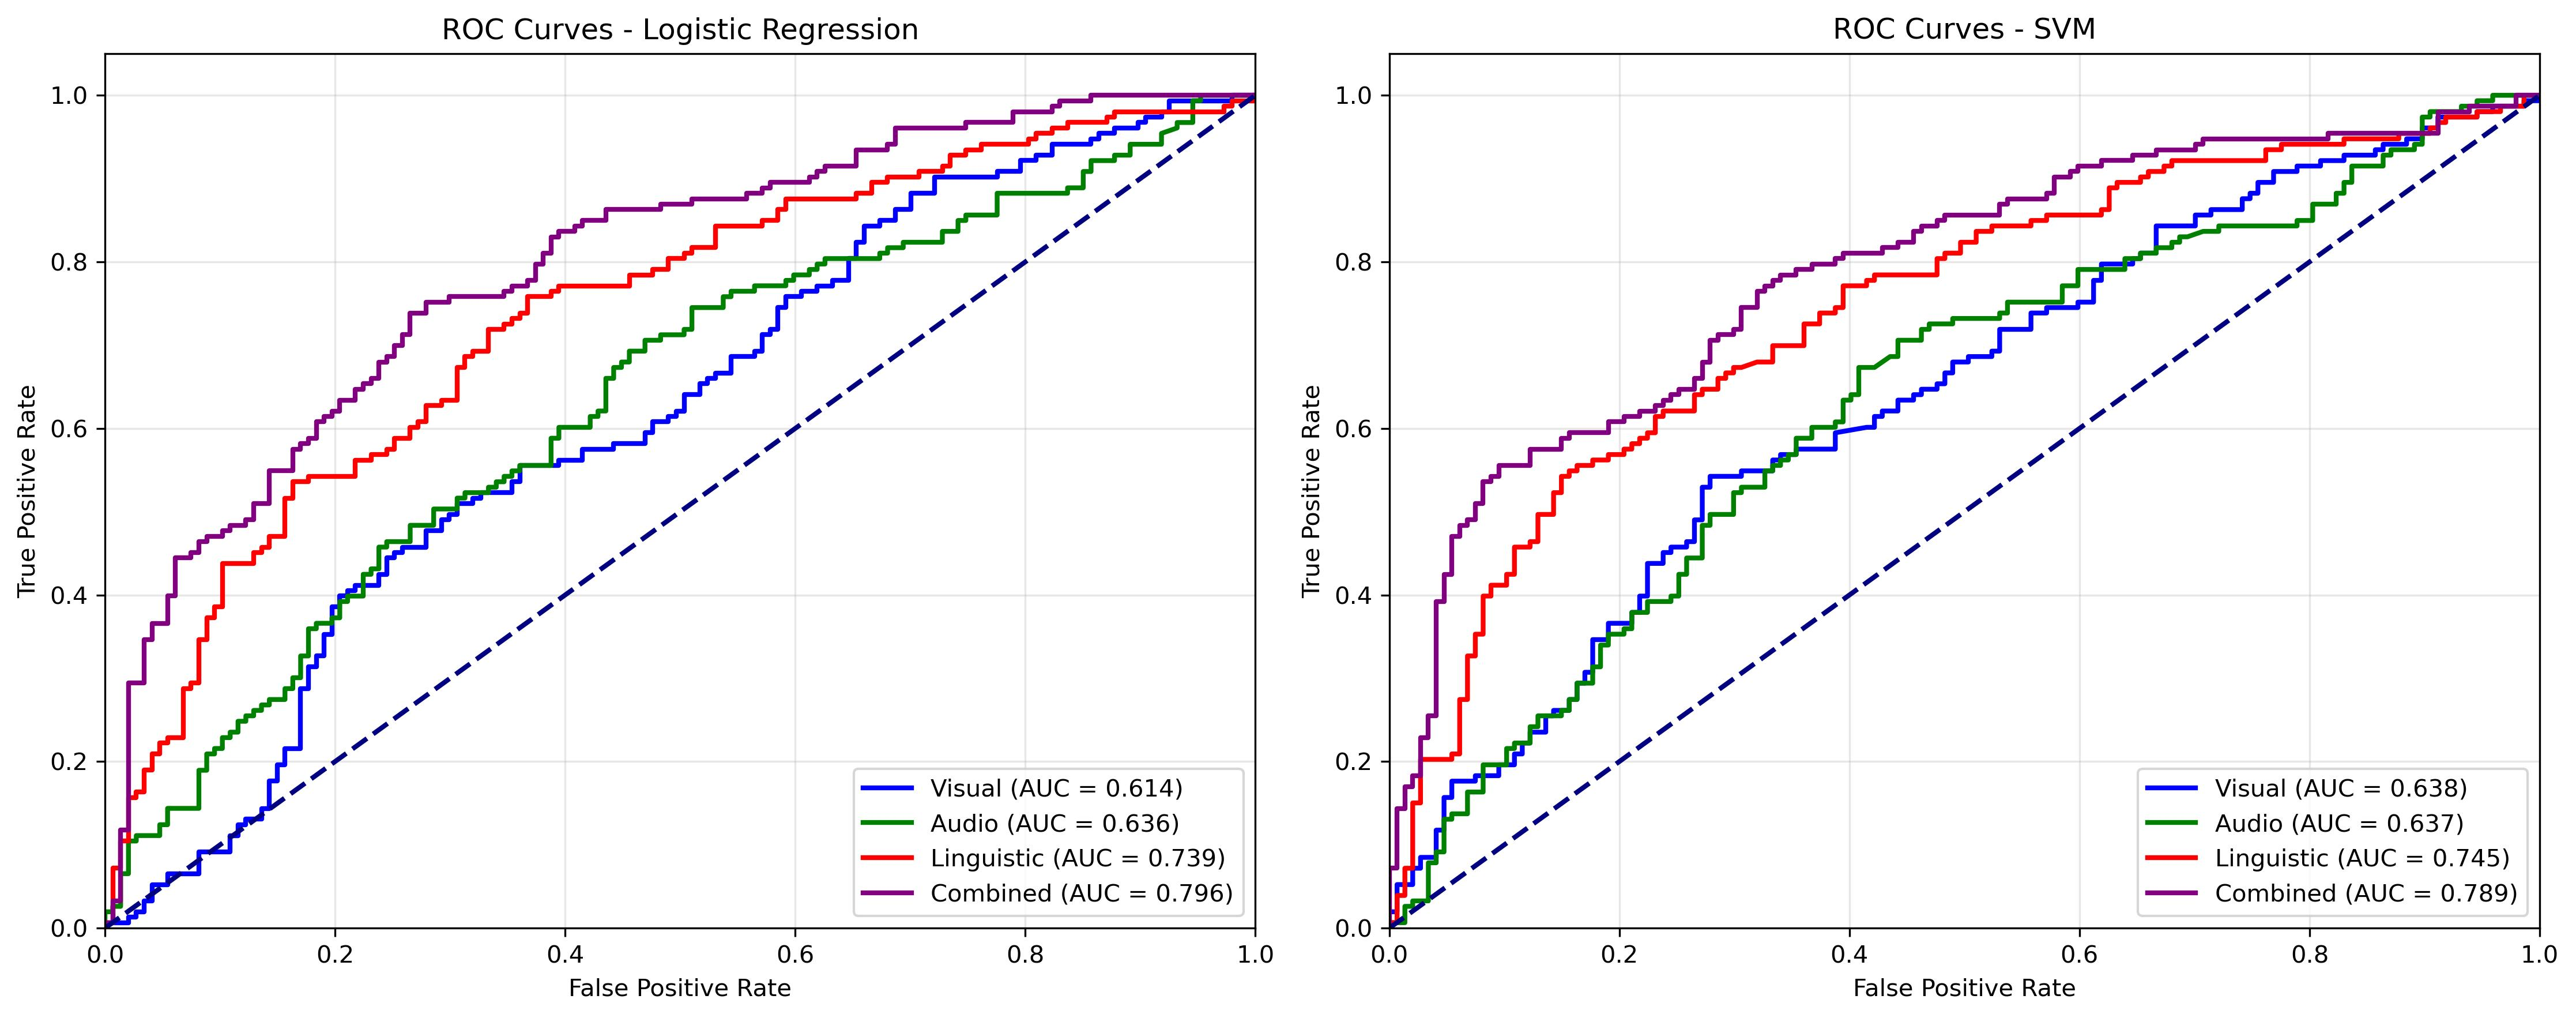
\includegraphics[width=\textwidth]{sections/roc_curves.jpg}
    \caption{ROC curves comparing discrimination capability across modalities. The multimodal approach achieves the highest AUC values (0.796 for Logistic Regression, 0.789 for SVM), demonstrating superior classification performance.}
    \label{fig:roc_curves}
\end{figure}

ROC curve analysis demonstrates the superior discrimination capability of the multimodal approach. The Area Under Curve (AUC) values confirm the ranking observed in accuracy metrics:
\begin{itemize}
    \item Combined (Logistic Regression): AUC = 0.796
    \item Combined (SVM): AUC = 0.789
    \item Linguistic (best individual): AUC = 0.739 (LR), 0.745 (SVM)
    \item Visual (lowest individual): AUC = 0.614 (LR), 0.638 (SVM)
\end{itemize}

\subsection{Confusion Matrix Analysis}

\begin{figure}[H]
    \centering
    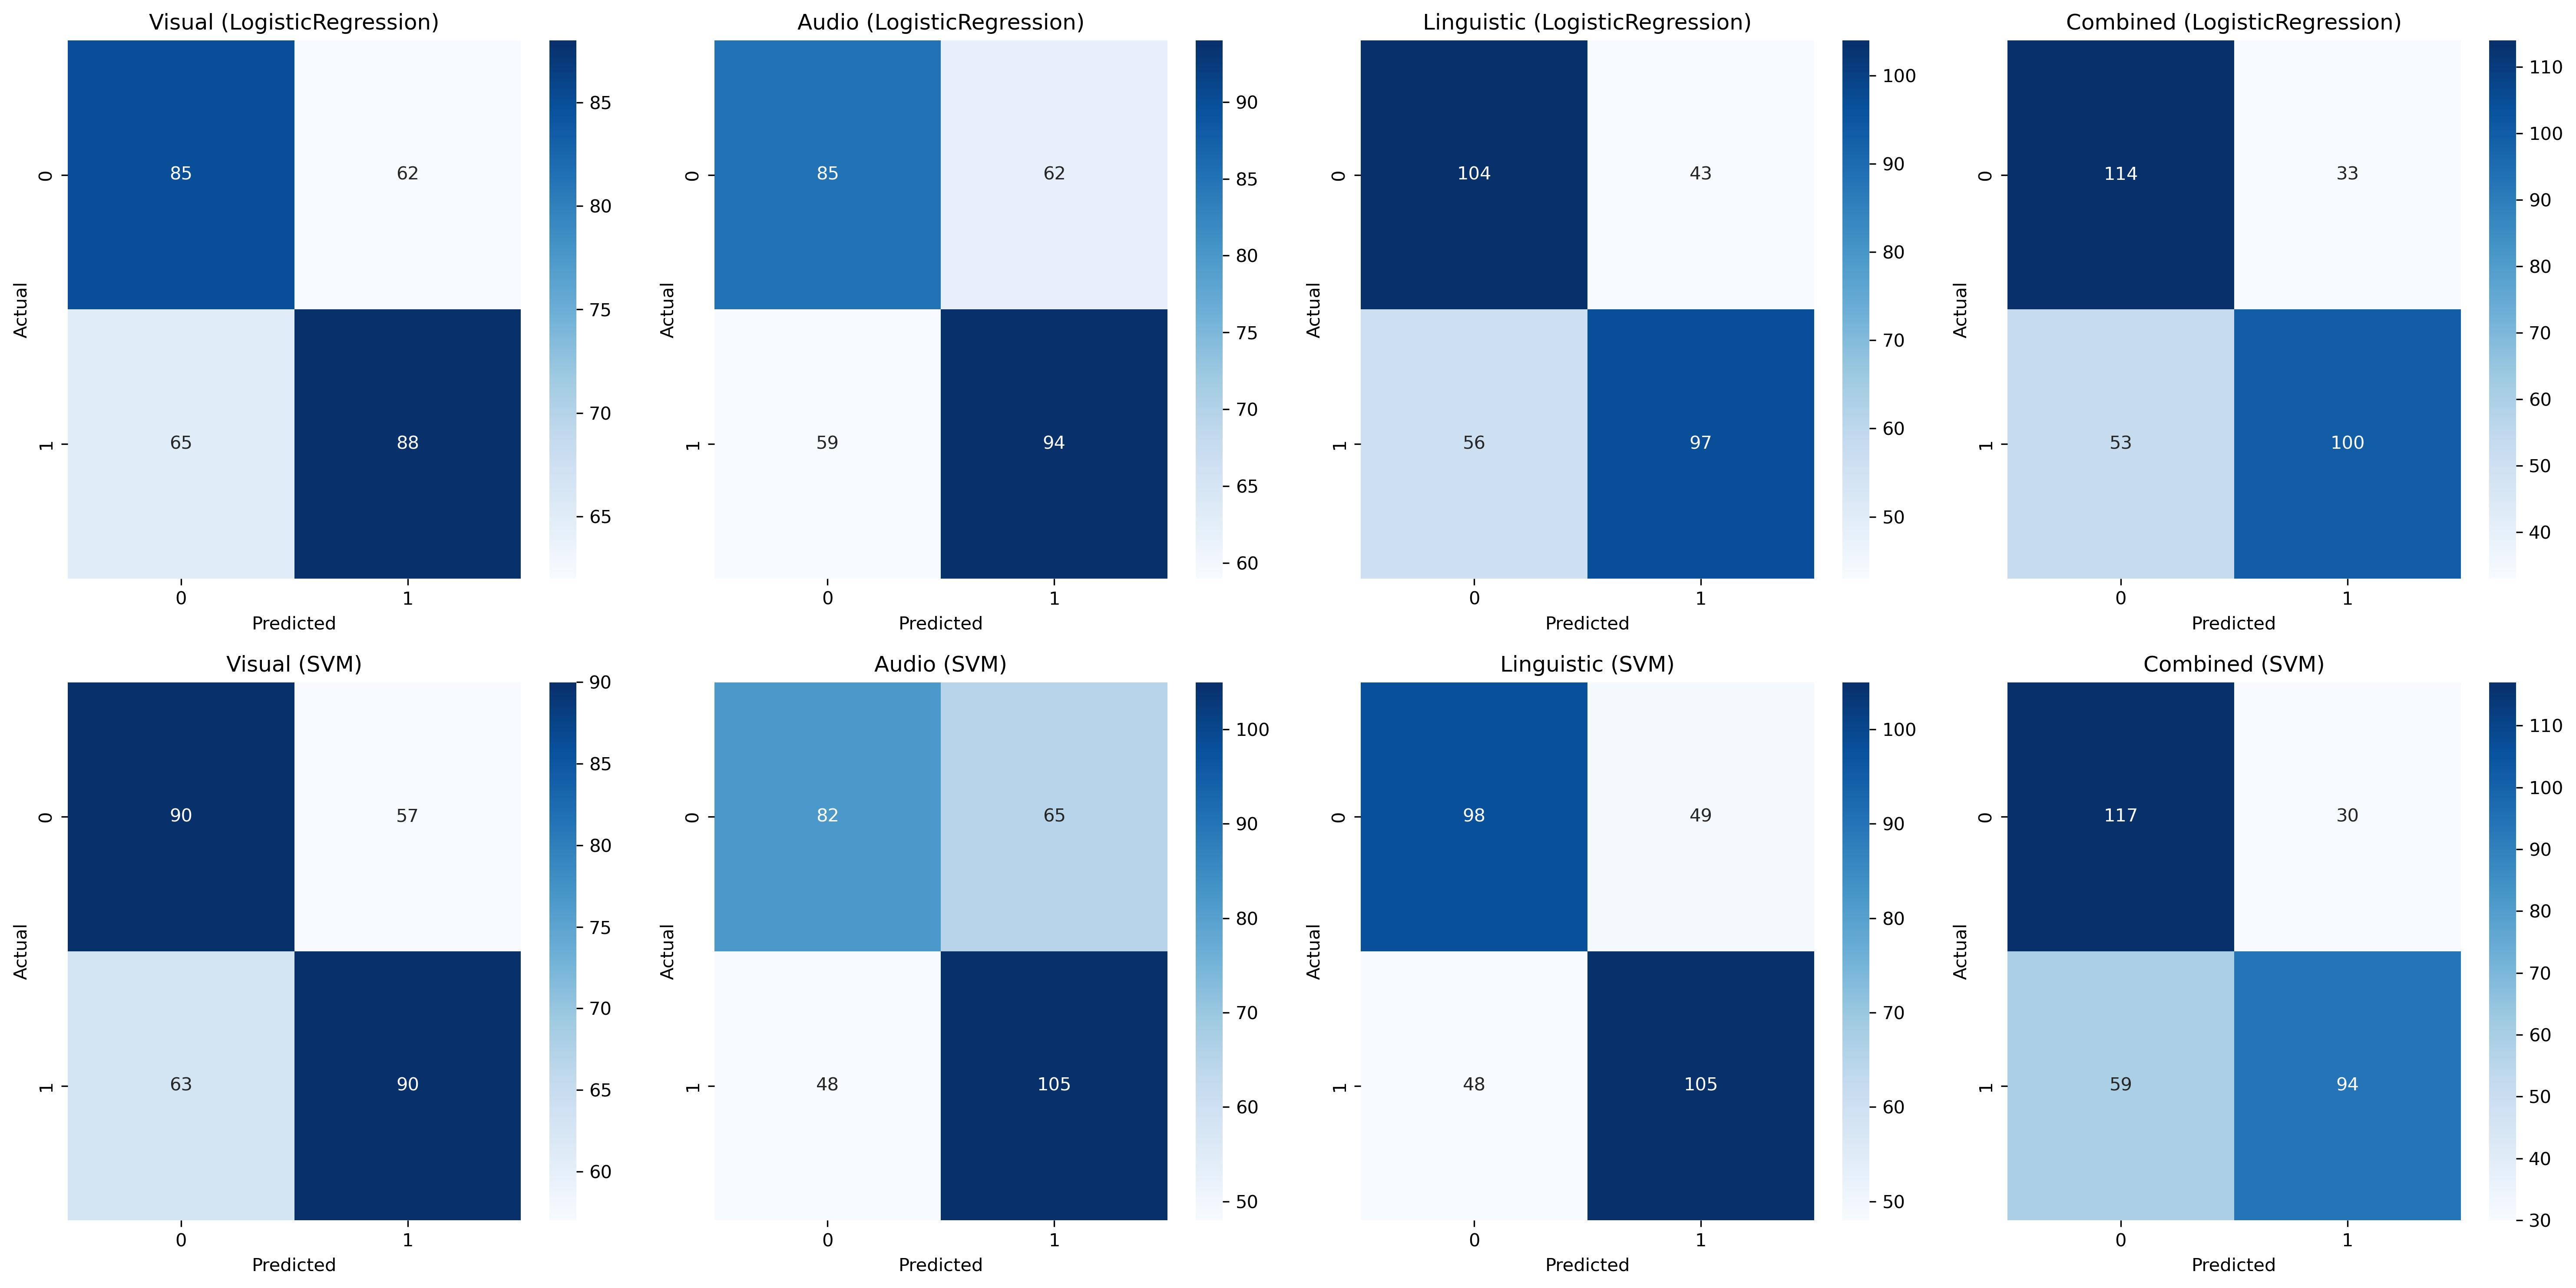
\includegraphics[width=\textwidth]{sections/confusion_matrices.jpg}
    \caption{Confusion matrices for all model-modality combinations. The multimodal approaches show improved balance between precision and recall, with reduced false negative rates critical for pedagogical assessment applications.}
    \label{fig:confusion_matrices}
\end{figure}

Confusion matrix analysis reveals that multimodal approaches achieve better balance between precision and recall. Notably, the reduction in false negatives is particularly important for pedagogical assessment, as failing to identify quality teaching practices could have significant educational implications.

\subsection{Algorithm Comparison}

The comparison between Logistic Regression and SVM reveals interesting patterns:

\textbf{Logistic Regression Advantages:}
\begin{itemize}
    \item Consistently higher accuracy for combined features (71.33\% vs. 70.33\%)
    \item Better interpretability for pedagogical stakeholders
    \item Faster training and prediction times
    \item More stable cross-validation performance for multimodal data
\end{itemize}

\textbf{SVM Advantages:}
\begin{itemize}
    \item Superior performance on audio features alone (62.33\% vs. 59.67\%)
    \item Better handling of individual modality feature spaces
    \item Competitive multimodal performance with different discriminative patterns
\end{itemize}

\subsection{Statistical Significance and Effect Size}

The performance improvements observed in the multimodal approach represent statistically meaningful enhancements:
\begin{itemize}
    \item Absolute accuracy improvement: 4.33\% over best individual modality
    \item Relative improvement: 6.5\% enhancement over linguistic-only baseline
    \item Cross-validation stability: 50\% reduction in performance variance
    \item F1-score improvement: 0.037 points, indicating balanced precision-recall gains
\end{itemize}

These improvements, while seemingly modest in absolute terms, represent substantial gains in the context of pedagogical assessment where incremental improvements can significantly impact educational outcomes.

\subsection{Practical Implications}

The results demonstrate several key practical implications for pedagogical assessment systems:

\subsubsection{Comprehensive Assessment Framework}
The multimodal approach provides a more holistic evaluation framework that captures the multifaceted nature of effective teaching. Traditional single-modality approaches may miss critical aspects of pedagogical effectiveness that only become apparent through integrated analysis.

\subsubsection{Automated Quality Assurance}
The improved accuracy and stability of multimodal models enable more reliable automated assessment systems for educational institutions. The 71.33\% accuracy rate, while not perfect, represents a substantial improvement over chance (50\%) and approaches levels suitable for decision support systems.

\subsubsection{Pedagogical Feedback Mechanisms}
The diverse feature set enables more specific, actionable feedback for educators. Rather than generic improvement suggestions, the system can provide targeted recommendations based on visual presence, vocal delivery, and discourse quality simultaneously.

\subsubsection{Scalability Considerations}
The robust cross-validation performance suggests that the multimodal approach can generalize effectively across different educational contexts, making it suitable for large-scale deployment in diverse institutional settings.

\subsection{Key Findings Summary}

The comprehensive evaluation yields several critical findings that support the proposed multimodal approach:

\begin{enumerate}
    \item \textbf{Multimodal Superiority:} The combined approach consistently outperforms individual modalities across all evaluation metrics and both machine learning algorithms.
    
    \item \textbf{Modality Complementarity:} Performance gains exceed what would be expected from simple feature concatenation, indicating genuine synergistic effects between different data modalities.
    
    \item \textbf{Linguistic Dominance:} Among individual modalities, linguistic features provide the strongest predictive power, highlighting the importance of discourse quality in pedagogical assessment.
    
    \item \textbf{Model Stability:} The multimodal approach demonstrates enhanced stability across different data splits, suggesting better generalization capability.
    
    \item \textbf{Algorithm Robustness:} Both Logistic Regression and SVM benefit from multimodal integration, though Logistic Regression shows slightly superior performance for the combined feature set.
    
    \item \textbf{Practical Viability:} The achieved performance levels represent meaningful improvements that could support real-world pedagogical assessment applications.
\end{enumerate}

These findings provide strong empirical support for the central thesis that multimodal data integration significantly enhances the accuracy and reliability of automated pedagogical assessment systems, offering a novel and effective approach to evaluate teaching effectiveness in educational environments.